\chapter{Evaluation}
\label{ch:evaluation}

This chapter describes the experiments conducted to evaluate the RFID hardware and localisation accuracy of the system. Each experiment description consists of justification, setup, results, and analysis. Section \ref{sec:hardeval} presents tests of the RFID hardware that provide an understanding of the mapping between RSSI and distance. Then, section \ref{sec:syseval} details the experiments that check whether the problem, described in section \ref{sec:probdef}, is solved by the system. It also provides results in terms of localisation accuracy and how these compare to results of the related work.

\section{Hardware Evaluation}
\label{sec:hardeval}

This section presents the experiments conducted in attempt to correlate received signal strength indicator (RSSI) and distance. This was accomplished by positioning the RFID tag at increasing distances and recording RSSI measurements from the RFID readers. Distance measurements were marked by a tape measure and RSSI values were recorded using the \textsf{SerialConnection} class developed as part of the system (details in section \ref{sec:constread}). All experiments had taken place in two indoor environments, an apartment and a university computer laboratory. These places differ in the amount of open space and the number and placement of objects.

In indoor environments, the attenuation of a radio signal is strongly influenced by the physical effects of reflection, refraction, multipath and shadow fading. Following from that, in order to construct a more complete notion of the relationship between RSSI and distance, a number of experiments were carried out. These include how RSSI changed as distance increased at different orientations of the tag to the readers and elevations of the tag from the floor. In addition, the wall penetration and range capabilities of the hardware were evaluated. The following subsections describe these experiments.

\subsection{Range}

The aim of this experiment was to measure the range capabilities of the RFID equipment in an indoor environment. In addition, RSSI values were recorded as distance between the readers and tag increased. In the first part of the experiment, the devices were keeping a line of sight between each other. Then, the test was repeated by obscuring the tag with an object, in this case a large whiteboard, to determine if it was affecting the communication range of the devices and the RSSI values reported by the readers. The experiments were carried out for each of the readers in a computer laboratory that had a 13-meter-long stretch of open space. The results of these experiments are illustrated on Figure \ref{fig:13m}.

\begin{figure}[h]
	\begin{center}
		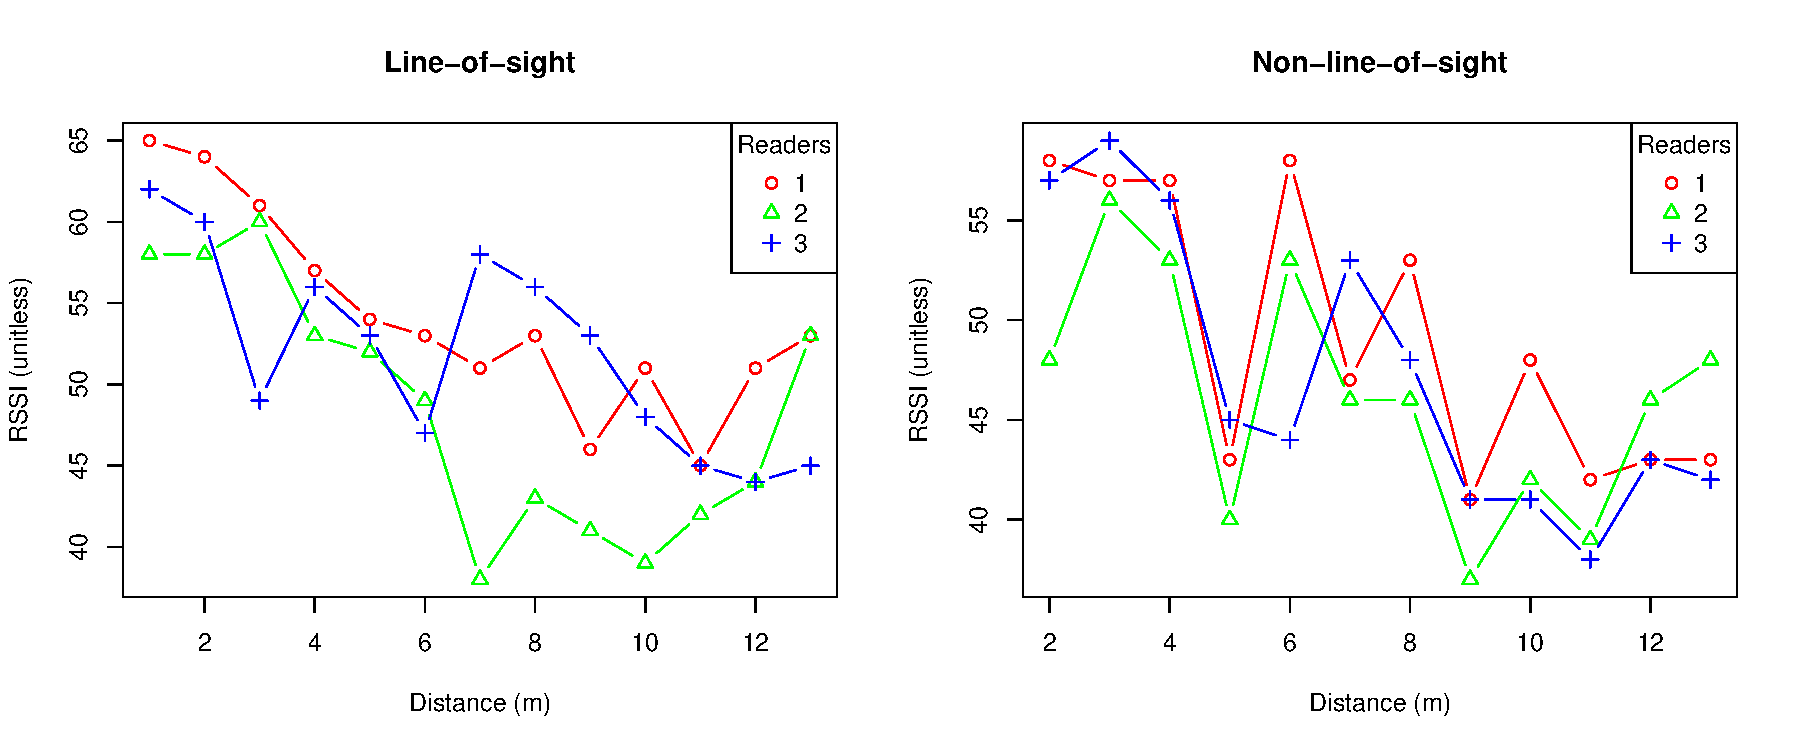
\includegraphics[width=1\textwidth]{figures/rssi_distance_13m}
		\caption{Two plots of RSSI measurements at increasing distances. On the $x$-axis, the distances from one to 13 meters are shown. The $y$-axis is the RSSI range. Notice how the RSSI ranges differ between the plots. The left graph shows how RSSI values measured at the three readers change with a line-of-sight signal propagation. The right graph illustrates the same experiment but with a non-line-of-sight signal propagation - the tag is occluded by an object.}
		\label{fig:13m}
	\end{center}
\end{figure}

There are three observations that could be made by looking at these results. First, in both experiments all three readers were able to detect the tag when located 13 meters away. The manufacturer reported a transmission range of 8 meters. Consequently, the antenna, designed in this project, had definitely increased the transmission range of the RFID tag. 

Second, these experiments confirm that the readers measure different RSSI for the same distance. As distance increases, the average difference between RSSI values is 4.93. The ranges on the $y$-axis are between 20 and 30 RSSI. Following from that, if the measurements reported by the readers differ in an average of around five units given the above ranges, then these readers are not calibrated to each other. This was observed in subsequent experiments as well. It was the motivation for constructing separate translation tables when mapping RSSI to distance.

Third, it is known that radio signals suffer from the effects of various physical phenomena when propagating in indoor environments. This was seen in all experiments when evaluating the RFID devices. Figure \ref{fig:13m} clearly shows that RSSI measurements do not decrease steadily and often fluctuate as the distance increases. This could be contributed to the characteristics of indoor spaces, where the shape of the space and the objects in it could cause reflection, refraction, and absorption of radio signals. Introducing an object that occluded the RFID tag had definitely decreased the RSSI values reported by the readers. It also caused the measurements to vary in unexpected ways.

\subsection{Line-of-sight Grid RSSI}

\begin{figure}[H]
	\begin{center}
		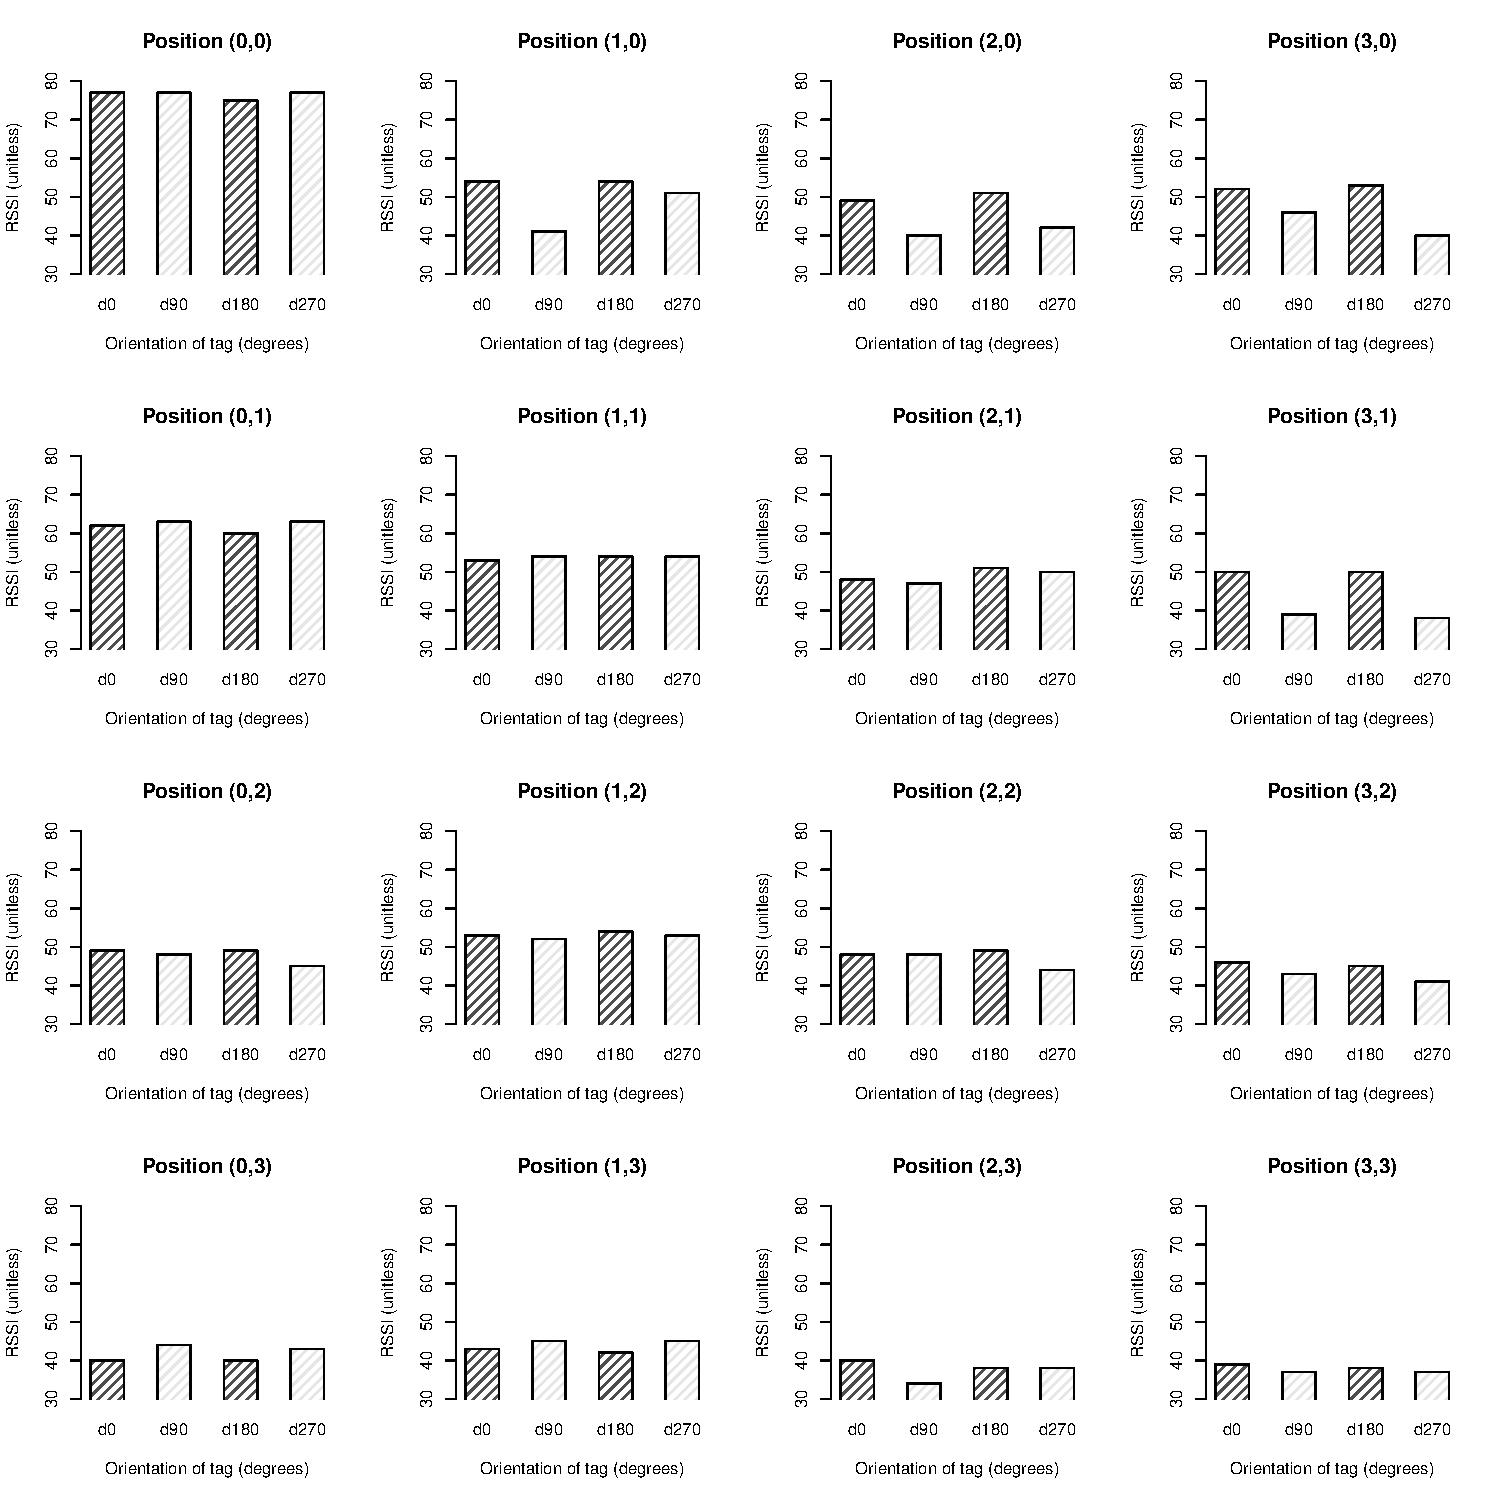
\includegraphics[width=1\textwidth]{figures/rssi_distance_grid_r1}
		\caption{Sixteen plots are organised into a four by four grid. Each plot represents the RSSI measurements of the \textbf{first} reader when the tag is placed at different positions on the x and y axes of the grid. The positions of the tag are all measured in meters. Every four bars in each plot show the RSSI readings when the tag is facing right (0\textdegree), up(90\textdegree), left (180\textdegree), and down (270\textdegree).}
	\end{center}
\end{figure}

\subsection{Orientation of tag to reader}

Conducted an experiment with the 3 readers and the active tag. Goal: to observe how the RSSI is changing as the tag moves away from a reader. Experimental setup: For every reader the tag is placed next to it, then 0.5m, 1m, 1.5m, 2m, 2.5m, and 3m away from the reader. For every distance the RSSI is recorded when there is a direct line of sight between the reader and the tag but also when the direct line of sight is obscured by some object (a suitcase filled with stuff). This is done for every reader and for every orientation of the reader (0, 45, 90, 135, 180, 225, 270, 315) to see if the readings get affected by the orientation of the reader. As a result, we get 8 tables (1 for every orientation) consisting of readings from the 3 readers once with a direct line of sight and once with an obscured line of sight (6 columns). These tables have 7 rows (1 for each distance). The results will be plotted and included in the final report where there will be a discussion of the implications of these results.

\begin{figure}[h]
	\begin{center}
		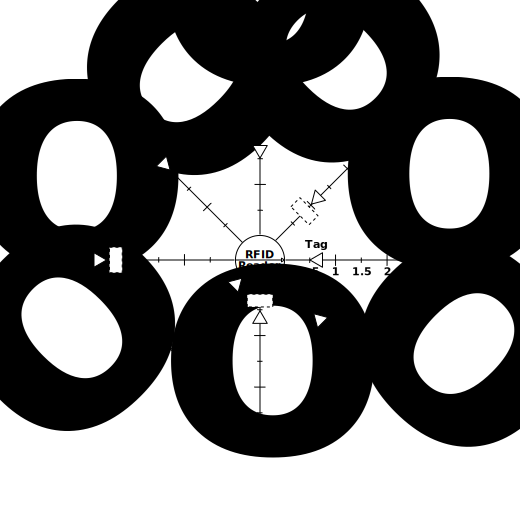
\includegraphics[width=.8\textwidth]{figures/exp/orientation}
		\caption{}
		\label{fig:ori}
	\end{center}
\end{figure}

\begin{figure}[H]
	\begin{center}
		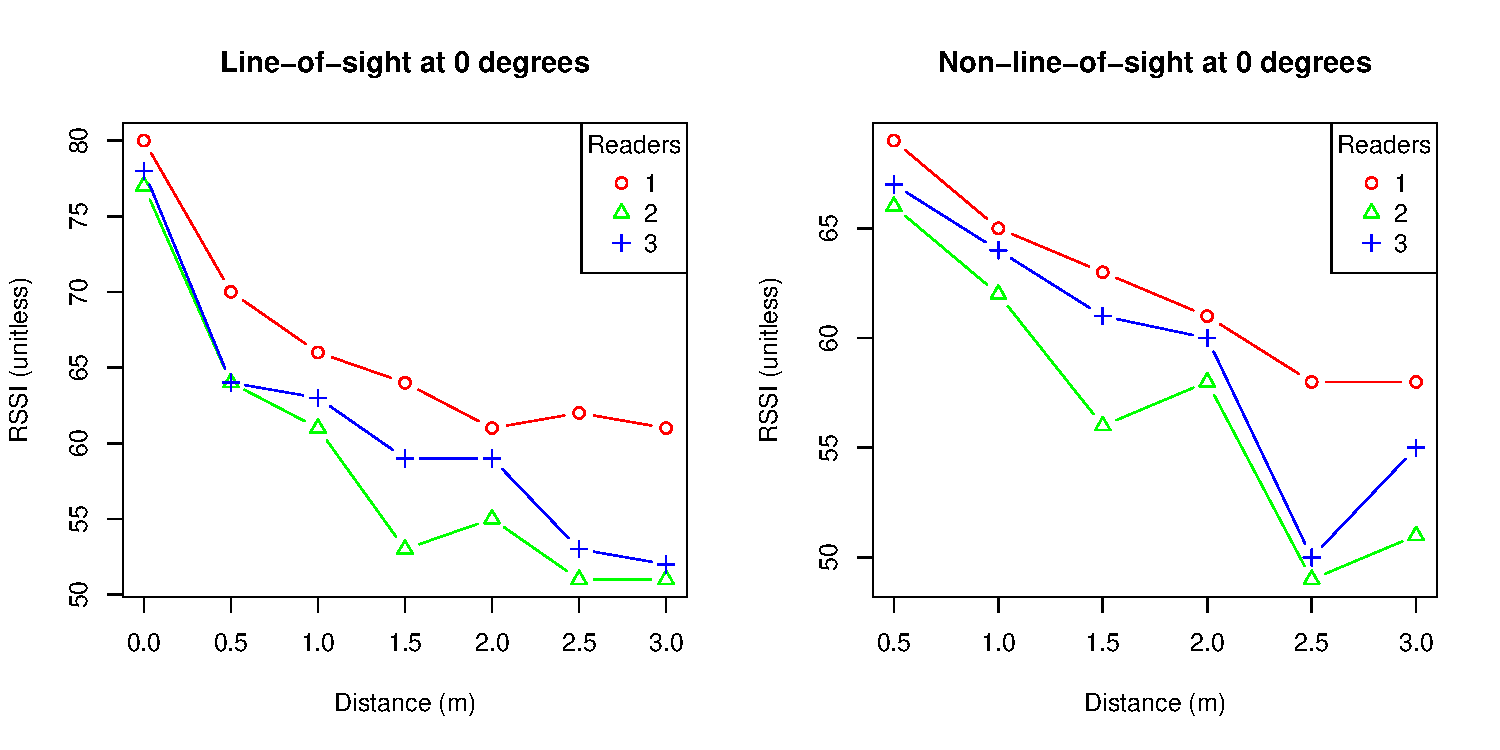
\includegraphics[width=1\textwidth]{figures/rssi_distance_3m_0deg}
		\caption{Two plots of RSSI measurements at increasing distances with the readers at 0 degrees (antennas facing the tag). The left graph show how RSSI values change with a line-of-sight signal propagation. The right graph illustrates the same experiment but with a non-line-of-sight signal propagation (there is an obstacle between the reader and the tag).}
	\end{center}
\end{figure}



\begin{figure}[H]
	\begin{center}
		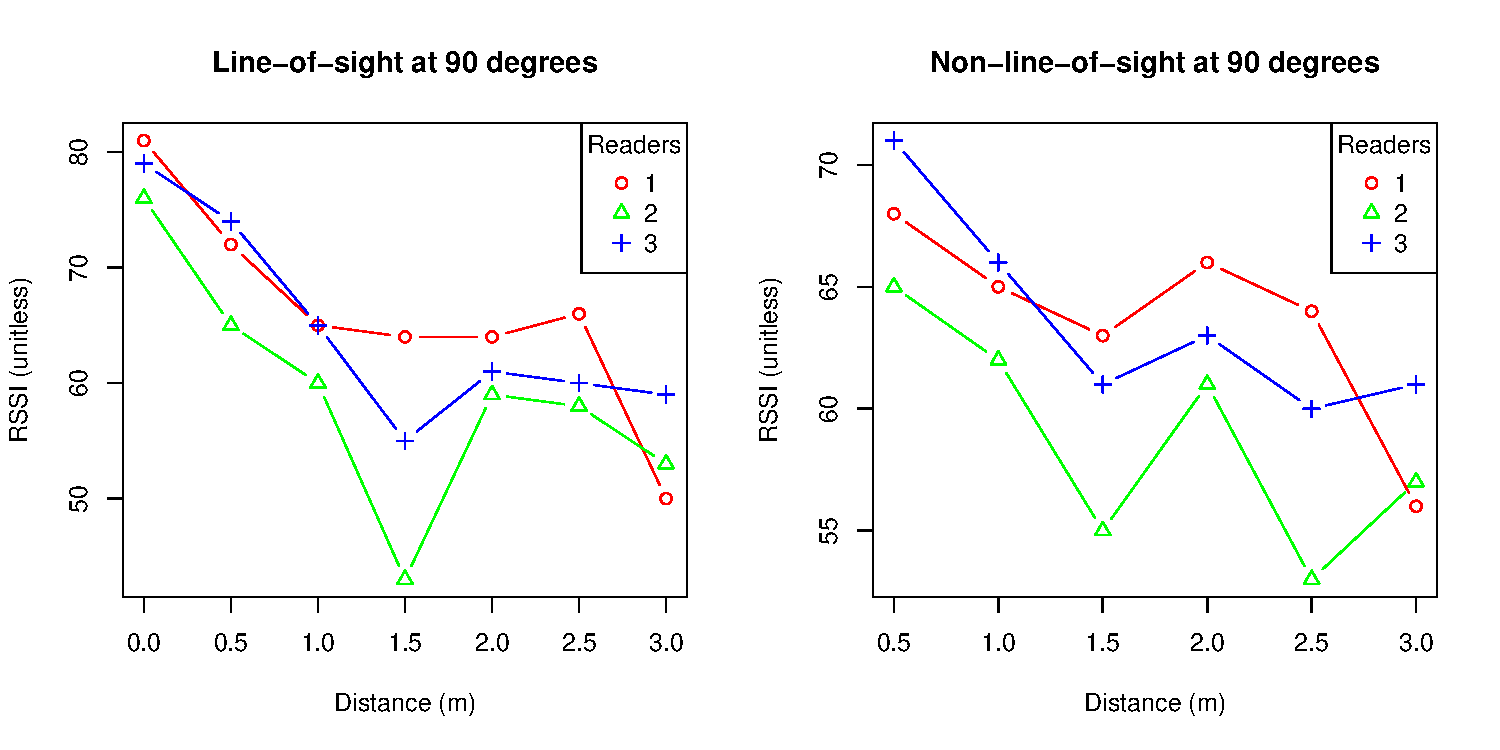
\includegraphics[width=1\textwidth]{figures/rssi_distance_3m_90deg}
		\caption{Two plots of RSSI measurements at increasing distances with the readers at 90 degrees (antennas at an angle to the tag). The left graph show how RSSI values change with a line-of-sight signal propagation. The right graph illustrates the same experiment but with a non-line-of-sight signal propagation (there is an obstacle between the reader and the tag).}
	\end{center}
\end{figure}


\subsection{Elevation}

Conducted an experiment with the 3 readers and the active tag. Goal: to measure if the position of the tag in height from the ground affects the RSSI. Experimental setup: The readers are positioned at floor level (6cm), at desk level (60 cm), and at 130cm. The tag is placed at the same heights at distances 1m, 1.5m, 2.0m, 2.5m, 3.0m, 3.5m, 4.0m. This results in a table with RSSI with 9 columns (3x for each reader at different heights) and 7 columns for each distance.

\begin{figure}[H]
	\begin{center}
		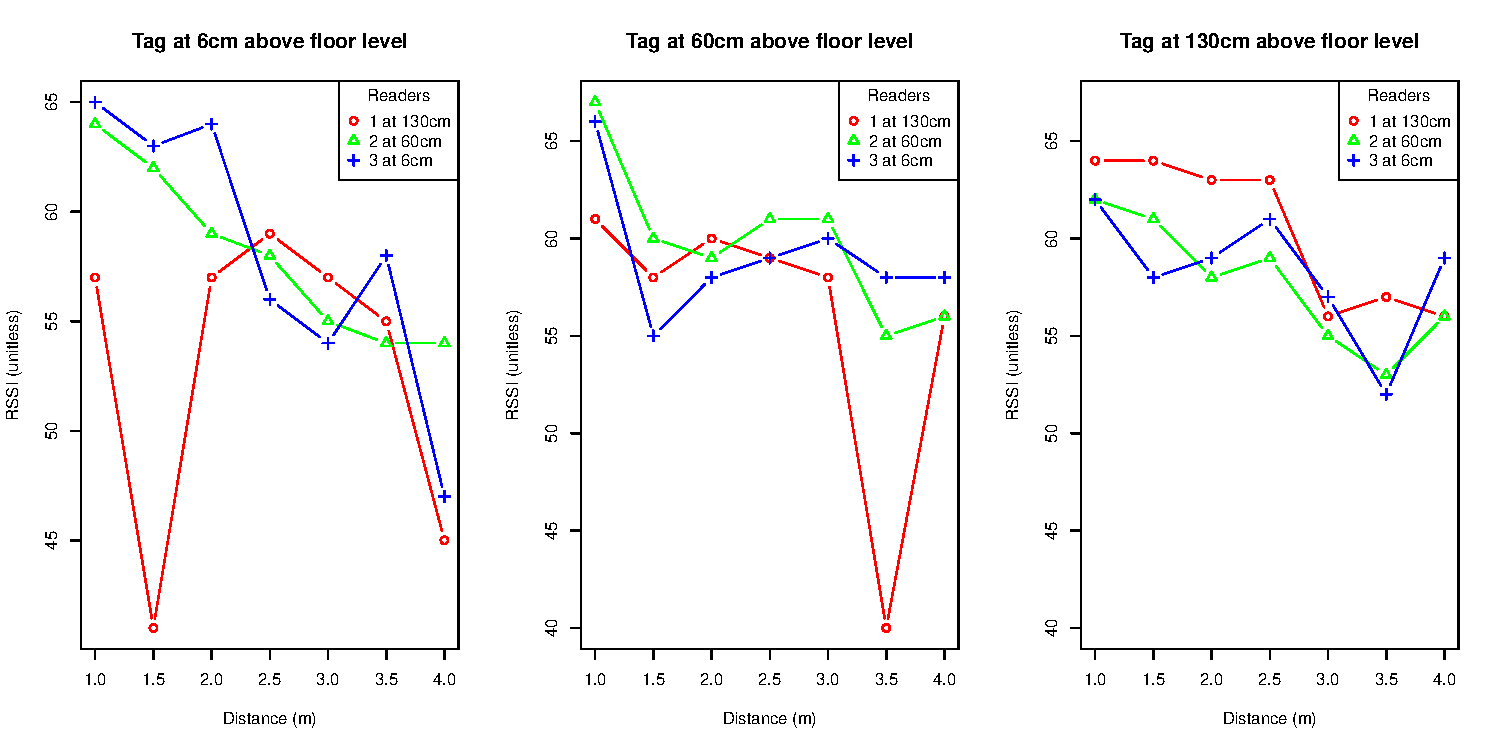
\includegraphics[width=1\textwidth]{figures/rssi_distance_4m}
		\caption{Three plots of RSSI measurements at increasing distances with the readers at different elevation from the floor in an indoor environment. The first graph shows how RSSI measurements change as the distance grows when the tag is placed at 6cm above floor level. The second and third graph show the same experiment but the tag is at 60cm and 130cm above the floor level.}
	\end{center}
\end{figure}


\subsection{Wall penetration}

Conducted an experiment with one reader and the active tag. Goal: to see the penetration capabilities of the tag/transmitter. Experimental setup: The reader was placed in one room, the tag in the adjacent room separated by a thin wall. The distance apart was 3m and RSSI: 41. Then I moved the tag in the next room adjacent to the previous so that the straight line between tag and reader is preserved. The tag was read at 4.8m distance with RSSI: 51. In the same room the tag was moved at the furthest possible position in the room at 8.2m with RSSI: 40. Then I got outside and went behind the building. The tag was read behind a 3rd thicker wall at distance 8.6m with RSSI: 32.

\section{System evaluation}
\label{sec:syseval}

By "mapping" I meant that the experiments check whether the problem is solved by the system, i.e. whether they give us a reliable way of checking the hypothesis. 

\subsection{Line-of-sight Grid Error}

Conducted a experiment in AT 3.01 (Robotics Lab). I took all the equipment, which fits into my backpack. I cleared a space 3 by 3 meters with no obstacles (line-of-sight propagation). Placed the reader nodes at 3 of the sides of the forming grid. Then I connected the whole system and powered it up. In this space, I placed markers every meter, thus forming a grid with 16 possible positions to place the tag. I did RSSI measurements at each position and also rotating the tag by 90 degrees. This resulted in 3 tables of RSSI measurements, one per reader. Each table consists of 16 cells, one for every position. Every cell has four RSSI values for different orientations of the tag. I also constructed a table with error measurements for every orientation of the tag. The error is a positive value in meters for both x and y axes reflecting the difference between real and estimated positions. 

\begin{figure}[H]
	\begin{center}
		
\includegraphics[width=1\textwidth]{figures/error_distance_grid}
		\caption{Sixteen plots are organised into a four by four grid. The readers are placed at positions (0,0), (0,3), and (3,0). Each plot represents the error in meters between measured and estimated location when the tag is placed at different positions on the grid. Each plot consists of four ellipses that illustrate the x and y error when the tag is facing right (0\textdegree), up(90\textdegree), left (180\textdegree), and down (270\textdegree). The colours of the ellipses are red, green, blue, and black, respectively.}
	\end{center}
\end{figure}

\begin{figure}[H]
	\begin{center}
		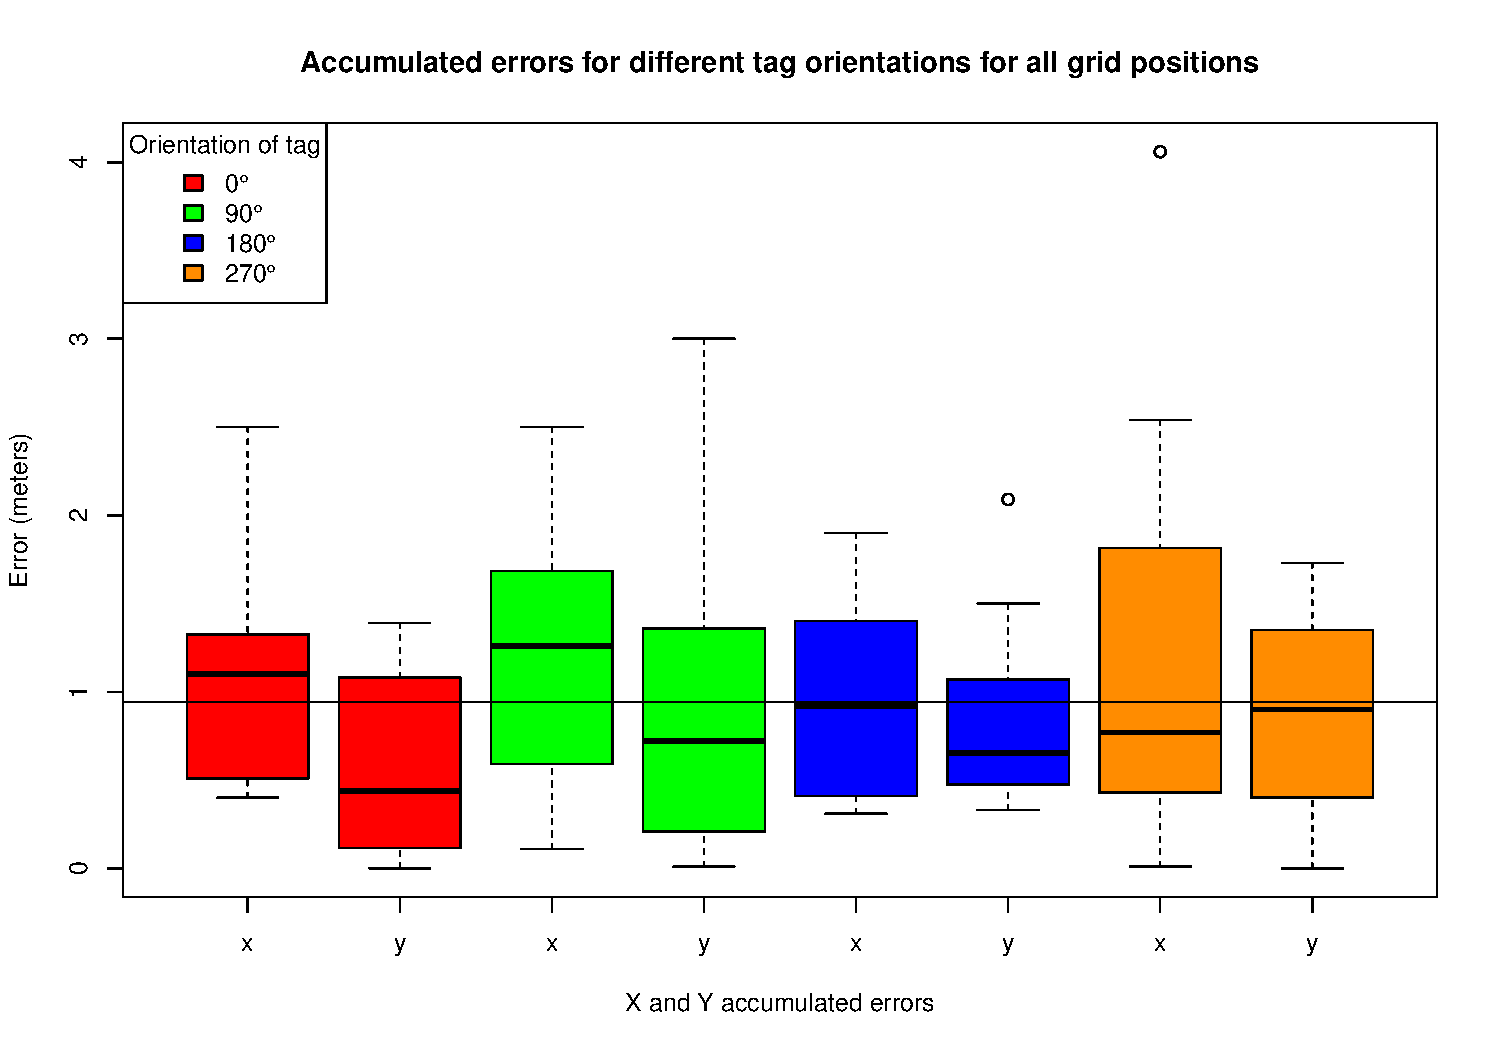
\includegraphics[width=1\textwidth]{figures/error_boxplot}
		\caption{A box plot showing errors between measured and estimated locations. The boxes are organised in four groups. Each group consists of errors in the x and y axes for a particular orientation of the tag. The horizontal line across the plot is the mean of all errors regardless of the tag orientation.}
	\end{center}
\end{figure}

\section{Discussion}

\section{Summary}
